\section{Лекция 5.Полярные конусы}
\subsection{Определение}
\noindent\textbf{Определение 2.33} \\

 Для конуса $K\subseteq \mathbb{R}^n$ полярным конусом называется множество
 \begin{equation*}
K^{\circ}:= \left\lbrace y \in \mathbb{R}^n : \left\langle y, x \right\rangle \leq 0  \text{, } \forall x \in K \right\rbrace
 \end{equation*}
 \begin{center}
 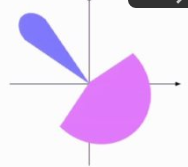
\includegraphics[scale=0.8]{image11.png}
 \end{center}
 \subsection{Свойства полярных конусов}
\begin{itemize}
\item \noindent\textbf{Замечание 2.34} Если $K_{1} \subseteq K_{2}$, то $K_{2}^{\circ} \subseteq K_{1}^{\circ}$
\item \noindent\textbf{Замечание 2.35} Для конуса $K\subseteq \mathbb{R}^n$ $cl(K)$ является конусом, что выполнятеся $K^{\circ}=(cl(K))^{\circ} $
\item \noindent\textbf{Замечание 2.36} Полярный конус является выпуклым замкнутым конусом.
\item \noindent\textbf{Замечание 2.37} Для $X\subseteq \mathbb{R}^n$ выполняется
\begin{equation*}
(cconeX)^{\circ}=\left\lbrace y \in \mathbb{R}^n | \left\langle x,y \right\rangle \leq 0 \text{, } \forall x \in X \right\rbrace
\end{equation*}
\end{itemize}
\noindent\textbf{Теорема 2.38} Для любого замкнутого выпуклого конуса $K$ выполняется $K^{\circ \circ}= K$\\
$\blacktriangleleft$
\begin{itemize}
\item  Очевидно, что $K\subseteq K^{\circ \circ}$.
\item  Допустим, что $y \in K^{\circ \circ} \setminus K$
\item  Т.к. $K$ замкнутый и выпуклый конус:\\ \\
\textbf{По Теореме 2.23}:
\begin{equation*} \tag{1}
\Longrightarrow \exists a\in\mathbb{R}^{n} \setminus \left\lbrace \mathbb{O}^{n} \right\rbrace :
\left\langle a,x \right\rangle \leq 0 \text{, } \forall x \in K
\end{equation*}
\begin{equation*} \tag{2}
\left\langle a,y \right\rangle = 1 > 0
\end{equation*}
\item Из (1) $\Longrightarrow a \in K^{\circ}$
\item Из (2) и того, что $y \in K^{\circ \circ} \Longrightarrow a \notin K^{\circ}$
\end{itemize}
Получили противоречие.
$\blacktriangleright$
\subsection{Поляр пересечений}
\noindent\textbf{Теорема 2.39}\\
Если $K_1, . . . , K_{q} \subseteq \mathbbm{R}^{n}$ - выпуклые конусы и
\begin{equation*} \tag{1}
 K_1 \cap \left(\cap_{i=2}^{q} int(K_{i})\right) \neq \varnothing \text{,}
\end{equation*}
тогда
\begin{equation*} \tag{2}
 \left(\cap_{i=1}^{q}{K_{i}}\right)^{\circ} = \sum_{i=1}^{q}{K_i}^{\circ}
\end{equation*}
где $int(X)$ - множество внутренних точек из $X\subseteq\mathbbm{R}^{n}$.\\
\textbf{Мотивация теоремы 2.39}
\begin{center}
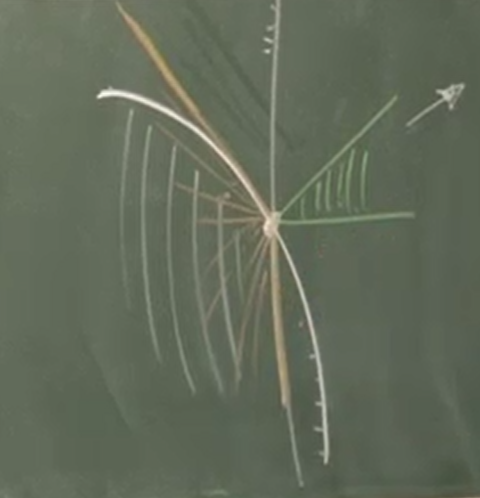
\includegraphics[scale=0.5]{image21.png}
\end{center}
\begin{itemize}
\item $K_{k}^{\circ} \subseteq \left(\cap_{i=1}^{q} K_{i}\right)^{\circ}\text{, } \forall k \in \left[ q \right]$
\item Т.к. $\left(\cap_{i=1}^{q} K_{i}\right)^{\circ}$ -- выпуклый конус $\Longrightarrow \sum_{k=1}^{q} K^{\circ} \subseteq \left(\cap_{i=1}^{q} K_{i}\right)^{\circ}$
\item $\left(\cap_{i=1}^{q} K_{i}\right)$ -- очень небольшой конус, который содержит только все общие элементы всех конусов $\Longrightarrow$ у этого конуса огромный поляр, который будет содержать всю $\sum_{k=1}^{q} K^{\circ}$.
\end{itemize}
\textbf{Частный случай Теоремы 2.39}
\begin{center}
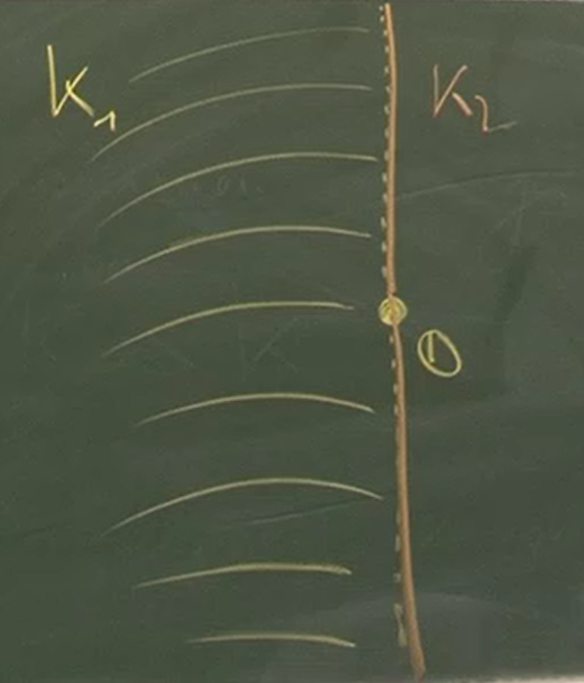
\includegraphics[scale=0.5]{image31.png}
\end{center}
\begin{itemize}
\item Первый конус задается как $K_{1}=\left\lbrace(0,0)\right\rbrace \cup \left\lbrace(x,y): x < 0\right\rbrace$
\item Второй конус: $K_{2}=\left\lbrace \left(0,y \right): y\in\mathbb{R}\right\rbrace$
\item Рассмотрим пересечение этих конусов:
\begin{equation*}
 K_{1}\cap K_{2} = \varnothing
\end{equation*}
\item Поляр пересеченеия равен всему пространству:
\begin{equation*}
\left( K_{1}\cap K_{2} \right)^{\circ} = \mathbb{R}^{2}
\end{equation*}
\item Поляр к первому конусу: $K_{1}^{\circ}=\left\lbrace(x,0): x\geq 0\right\rbrace$
\item Ко второму: $K_{2}^{\circ}=\left\lbrace(x,0): x\in\mathbb{R}\right\rbrace$
\item Сумма Минковского поляров: $K_{1}^{\circ} + K_{2}^{\circ}=\left\lbrace(x,0): x\in\mathbb{R}\right\rbrace$
\item Как видно, сумма Минковского полностью содержится в поляре пересечения.
\item Однако, теорема не выполняется в следствие того, что нарушены условия: пересечение проходит только по нулевому вектору.
\end{itemize}
Переходим к доказательству теоремы 2.39:
$\blacktriangleleft$\\
"$\supseteq :$"  Очевидно, смотри мотивацию к теореме.
\\
"$\subseteqq :$"  Необходимо показать, что поляр содержится в сумме Минковского:
\begin{itemize}
    \item Это, очевидно, выполняется для нулевого вектора:
\begin{center}
    $0\in\sum_{i=1}^{q}{K_i}^{\circ}$
\end{center}

\item Достаточно для каждого $y\in(\bigcap_{i=1}^{q}{K_i})^{\circ} \diagdown \{0\}$ показать, что \begin{center}
    $y\in\sum_{i=1}^{q}{K_i}^{\circ}$
\end{center}

\item Определим множество $K_0:=\{x\in \mathbbm{R}^{n} :\langle y,x\rangle>0\}$. Данное монжество выпукло и замкнуто.

\item Зададим 2 выпуклых множества: \\
\begin{center}
    $ \mathcal{K} := K_0* K_1* \ldots * K_{q}$,
\end{center}
Где $\mathcal{K}\subseteq\mathbbm{R}^{(q+1)n}$.\\
\begin{center}
    $ \mathcal{D} := \{(x,x,x,\ldots,x)\in \mathbbm{R}^{(q+1)n} : x\in \mathbbm{R}^{n} \}\subseteq\mathbbm{R}^{(q+1)n}$.
\end{center}
Эти множества являются выпуклыми ($\mathcal{K}$ является декартовым произведением выпуклых, а $\mathcal{D}$ -- линейной оболочкой, что тоже является выпуклым множеством), при этом $\mathcal{K}\bigcap\mathcal{D}=\varnothing$, т. к.:
\begin{itemize}
    \item Во множестве $K_{0}$ лежат только те вектора $x$, с которыми $\left\langle x,y \right\rangle >0$, а в $K_{i}, i\in \left\lbrace 1,...,q\right\rbrace$ лежат только такие векторы, которые дают неположительное скалярное произведеление с $y. \Longrightarrow$ В $\mathcal{K}$ не содержится элементов вида такого, как в $\mathcal{D}$.
\end{itemize}
\item \textbf{Из теоремы 2.16}:
\begin{center}
    $\exists a\in \mathbbm{R}^{(q+1)n} : \langle $a$,z\rangle \leq \langle a,\widetilde{z}\rangle$, для любого $z \in \mathcal{K}$ и $\widetilde{z} \in \mathcal{D}$.\\
    где $a=(y^{(0)}, y^{(1)}, \ldots, y^{(q)})\neq \mathbb{O}$.
\end{center}
Таким образом(отсюда надо проверять дальше):
\begin{center}
     $\forall X^{(0)}\in K_0,  X^{(1)}\in K_1, \ldots,  X^{(q)}\in K_q, \forall x\in\mathbbm{R}^{n}$
 $\sum_{i=0}^{q}{\langle y^{i},x^{i}\rangle} \leq \sum_{i=0}^{q}{\langle y^{i},x\rangle} = \langle \sum_{i=0}^{q}{y^{i}},x\rangle $ (*)
\end{center}
Не все  $y^{i}=0$, это гарантируется условием теоремы.
\item Из (*) следует, что:
\begin{center}
     $\exists M\in\mathbbm{R}:\forall i\in \{ 0,\ldots,q\}, \forall x^{(i)}\in K_{i} :\langle y^{i},x^{i}\rangle \leq M  $
отсюда следует, что
$\langle y^{i},x^{i}\rangle \leq 0, \forall x^{(i)}\in K_{i}, \forall i\in \{ 0,\ldots,q\} $
\end{center}
\item $y^{(i)}\in K_{i}^{\circ}, \forall i in\{0,1,\ldots,q\}$\\
Допустим, что $y^{(0)}=\alpha y$, где $\alpha\leq 0$.
Т.к. $y^{(0)}=\alpha y+u$ и $u\bot y$, т.е. $\langle y,u\rangle=0$

Возьмём  $\langle y^{(0)},u\rangle=\|u\|^2\succ 0$, тогда $\exists$ окрестность $U$ точки $u$, где $\langle y^{(0)},x\succ 0$, $\forall x\in U$. Получим противоречие, т. к. $U\bigcap K_0\neq\varnothing$.
Тогда $y^{(0)}=\alpha y, y\in K_0 -> 0\geq \langle y^{(0)},y\rangle=\alpha\|y\|^2, y\neq 0$

\item Из (*) следует, что:
\begin{center}
     $\exists L\in\mathbbm{R}: \forall x^{(i)}\in R^{L} :
\langle \sum_{i=0}^{u}{y^{i}},x\rangle \geq L,  \sum{y^{(i)}}=0 (**)$
\end{center}

\item Из (**)следует, что:
\begin{center}
    $-\alpha y=-y^{(0)}=\sum_{i=1}^{q}{y^{(i)}}\in \sum_{i=1}^{q}{K_i}$
\end{center}

\item $\exists x\in K_1\bigcap(\bigcap_{i=2}^{q}{int(K_i)})$
Предположим, что $\alpha =0$, то $y^(0)=0$, тогда в (**):
\begin{center}
    $\sum_{i=1}^{q}{y^{(i)}}=0$ (***)
\end{center}
Откуда следует, что:
 \begin{center}
    $\sum_{i=1}^{q}{\langle {y^{i}},x\rangle}=\langle \sum_{i=1}^{q}{y^{i}},x\rangle=0$
\end{center}
Откуда в свою очередь следует, что:
\begin{center}
    $\forall i\in\{1,\ldots,q\},\langle {y^{i}},x\rangle=0 (****)$
\end{center}
Сумма неположительных равна нулю.

\item Т. к. $x\in int K_i \forall i\in\{2,\ldots,q\}\exists \varepsilon\succ0
$
и $x+\varepsilon y^{(i)}\in K_i $

$\forall i\in\{2, \dots, q\} : 0\geq \langle {y^{i}},x+\varepsilon y^{(i)}\rangle= \langle {y^{i}},x\rangle+\varepsilon \|y\|^2\ $

Из этого следует, что все $y^{(i)}=0$
\end{itemize}

Получаем противоречие.

$\blacktriangleright$ 